\documentclass[aspectratio=169,10pt]{beamer}

\usetheme[progressbar=frametitle,noslidenumbers]{metropolis}
\usepackage{appendixnumberbeamer}

\usepackage{booktabs}
\usepackage[scale=2]{ccicons}

\usepackage{pgfplots}
\usepgfplotslibrary{dateplot}

\usepackage{xspace}
\newcommand{\themename}{\textbf{\textsc{metropolis}}\xspace}

\title{Frameworks, Tools and Workflows}
\subtitle{and their impact on science}
% \date{\today}
\date{\today}
\author{Lukas Pfahler}
\institute{TU Dortmund University, Chair for Artificial Intelligence}
\titlegraphic{\hfill
\includegraphics[height=8mm]{tu-do-logo.pdf}}

\begin{document}

\maketitle
\section{Setup}
\begin{frame}{Intention}
Goal of this DuD is to
\begin{itemize}
    \item present tools or frameworks you use frequently
    \item present how you use them: \textbf{Characteristic Workflows}
\end{itemize}
\end{frame}
% 1. Beitrag (Beispiel)
\section{Example Person}
% Let's start with an eye-catcher
\begin{frame}[fragile]{RapidMiner}
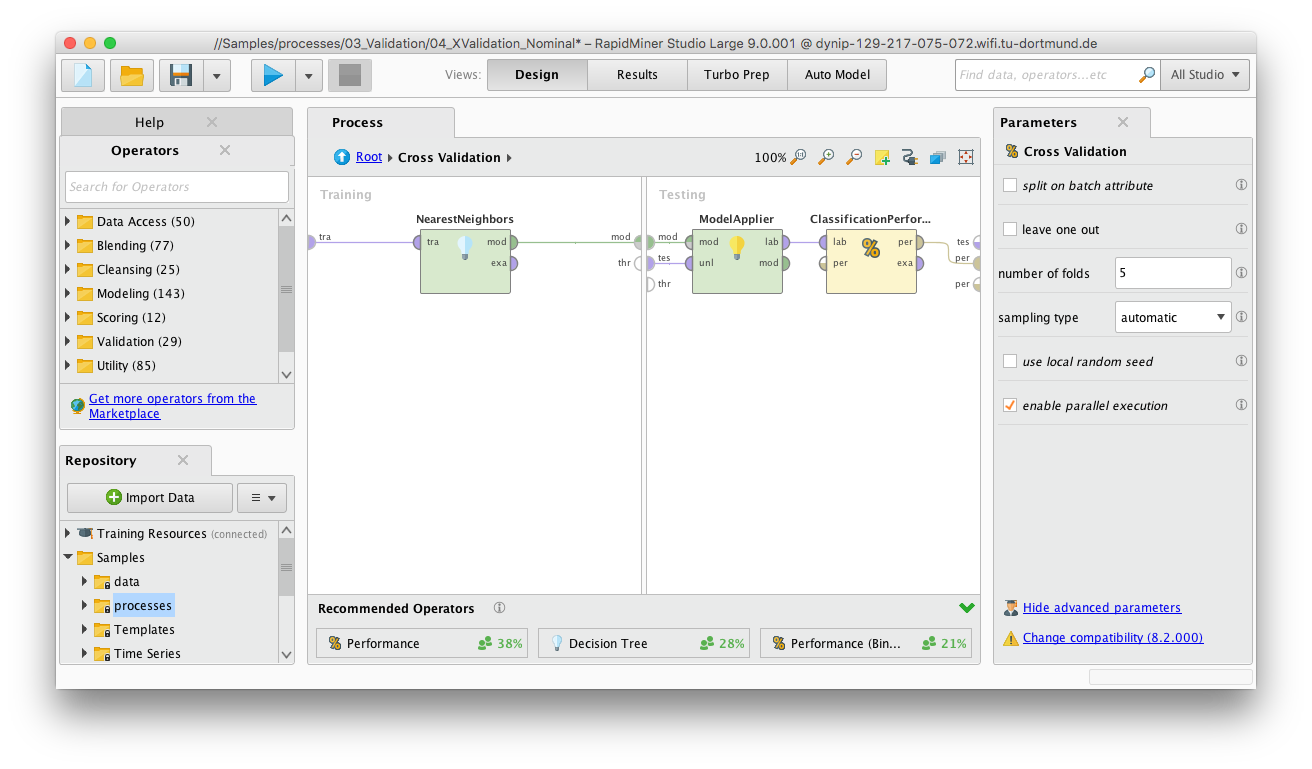
\includegraphics[width=\linewidth]{rapidminer.png}
\end{frame}
\begin{frame}[t,fragile]{Review}
    \begin{columns}[t]
    \begin{column}{0.5\textwidth}
    \begin{block}{Convenience}
        Has all the building blocks of routine machine learning tasks:
        \begin{itemize}
            \item Data Import
            \item Normalization
            \item Standard Machine Learning Methods
            \item Validation
            \item Visualization
        \end{itemize}
    \end{block}
    \end{column}
    \begin{column}{0.5\textwidth}
    \begin{block}{Reproducibility}
        Let's write some stuff
        \begin{itemize}
        \item Exchangable XML specifications of data mining processes
        \item No Version Control of Process Files $\rightarrow$ Manual Versioning via FileNames
        \end{itemize}
    \end{block}
    
    \end{column}
    \end{columns}
    \hfill
    
    \begin{alertblock}{Takeaway Message}
        Rapidminer offers you the possibility to quickly evaluate the performance of a wide range of standard methods on a new data mining task.
    \end{alertblock}
    
\end{frame}

\section{Amal}
\begin{frame}[fragile]{EyeCather}
\end{frame}
\begin{frame}[t,fragile]{Review}
\end{frame}

\section{Katharina}
\begin{frame}[fragile]{EyeCather}
\end{frame}
\begin{frame}[t,fragile]{Review}
\end{frame}

\section{Alexey}
\begin{frame}[fragile]{EyeCather}
\end{frame}
\begin{frame}[t,fragile]{Review}
\end{frame}

\section{Mirko}
\begin{frame}[fragile]{EyeCather}
\end{frame}
\begin{frame}[t,fragile]{Review}
\end{frame}

\section{Sebastian}
\begin{frame}[fragile]{EyeCather}
\end{frame}
\begin{frame}[t,fragile]{Review}
\end{frame}

\section{Lukas}
\begin{frame}[fragile]{EyeCather}
\end{frame}
\begin{frame}[t,fragile]{Review}
\end{frame}

\section{Sibylle}
\begin{frame}[fragile]{EyeCather}
\end{frame}
\begin{frame}[t,fragile]{Review}
\end{frame}

\section{Thomas}
\begin{frame}[fragile]{EyeCather}
\end{frame}
\begin{frame}[t,fragile]{Review}
\end{frame}
\end{document}
